% !TEX root = ../../main.tex


\begin{figure}[!htb]
\centering
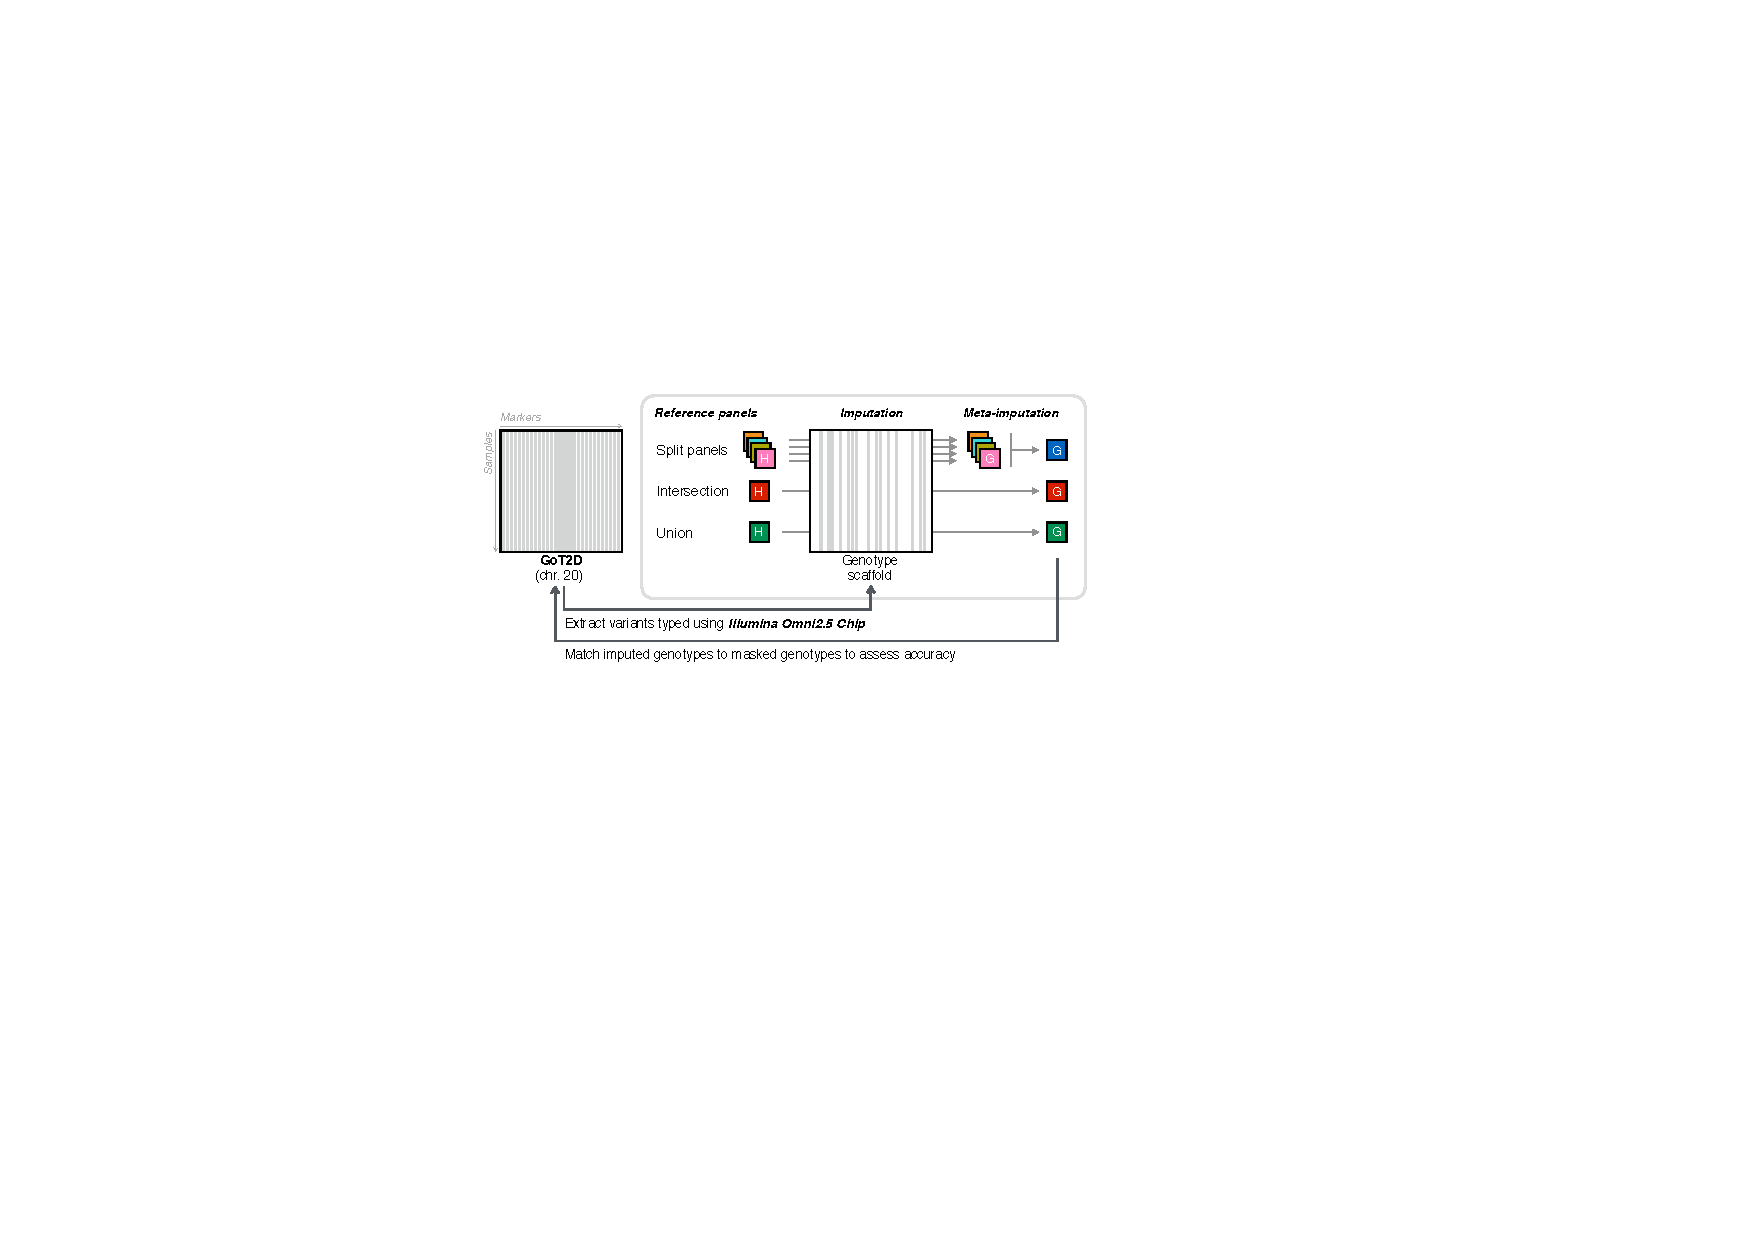
\includegraphics[width=0.9\textwidth]{./img/ch2/info_design_accuracy}
\Caption{Illustration of the accuracy assessment process}
{Imputations were performed on the same genotype scaffold, which consisted of genetic markers obtained through genotyping using \emph{Illumina Omni2.5 Chip}, which was part of the \gls{got2d} dataset.
This scaffold was extracted from \gls{got2d} data, where remaining markers were masked for subsequent calculation of accuracy (squared Pearson correlation coefficient, $r^2$) at corresponding sites after imputation.
Several reference panels were available, which were imputed into the same scaffold.
Meta-imputation was applied to the imputed datasets obtained from split panels, which were generated as distinct subsets from the \gls{1kg} dataset.
The intersection and union panels were separately imputed into the scaffold and subsequently compared to meta-imputed data on corresponding variant sets.}
{fig:info_design_accuracy}
\end{figure}
